% ============================================================================
% LLM-Powered Customer Churn Analysis with RAG and QLoRA Fine-Tuning
% NeurIPS-style Technical Report
% ============================================================================
\documentclass[10pt,letterpaper]{article}

% ── Packages ────────────────────────────────────────────────────────────────
\usepackage[margin=1in]{geometry}
\usepackage{times}
\usepackage{amsmath,amssymb,amsfonts}
\usepackage{graphicx}
\usepackage{booktabs}
\usepackage{hyperref}
\usepackage[numbers,sort&compress]{natbib}
\usepackage{pgfplots}
\pgfplotsset{compat=1.17}
\usepackage[ruled,vlined,linesnumbered]{algorithm2e}
\usepackage{multirow}
\usepackage{xcolor}
\usepackage{enumitem}
\usepackage{float}
\usepackage{caption}
\usepackage{subcaption}
\usepackage{tabularx}

% ── Hyperref setup ──────────────────────────────────────────────────────────
\hypersetup{
    colorlinks=true,
    linkcolor=blue!70!black,
    citecolor=blue!70!black,
    urlcolor=blue!70!black,
}

% ── Custom commands ─────────────────────────────────────────────────────────
\newcommand{\method}{\textsc{ChurnRAG}}

% ── Title ───────────────────────────────────────────────────────────────────
\title{LLM-Powered Customer Churn Analysis \\ with Retrieval-Augmented Generation and QLoRA Fine-Tuning}

\author{
    Ricky Gong \\
    \texttt{gong8@seas.upenn.edu}
}

\date{}

\begin{document}
\maketitle

% ============================================================================
% ABSTRACT
% ============================================================================
\begin{abstract}
Customer churn prediction and analysis remain critical challenges in the telecommunications industry, where the average monthly churn rate of 1.5--2\% translates to an estimated \$65 billion in annual revenue loss in the United States alone. Traditional machine learning approaches to churn prediction focus on binary classification but fail to provide the interpretable, actionable analysis that business stakeholders require. In this paper, we present \method{}, an end-to-end system that combines Retrieval-Augmented Generation (RAG) with QLoRA fine-tuning of open-source large language models for comprehensive customer churn analysis. Our system employs a hybrid retrieval pipeline combining dense vector search with BM25 keyword matching via Reciprocal Rank Fusion, paired with the Qwen2.5-7B-Instruct model quantized to 4-bit NormalFloat (NF4) precision. We introduce a teacher-student distillation pipeline using Qwen2.5-14B-Instruct to generate 305 high-quality domain-specific training samples, enabling QLoRA fine-tuning on a single consumer GPU. To address post-fine-tuning regressions in citation accuracy and risk assessment consistency, we propose a hybrid inference pipeline that augments LLM generation with deterministic post-processing for citation validation and mathematical risk scoring. Our improved pipeline achieves 100\% JSON format compliance, 100\% citation accuracy, and consistent risk level alignment across all evaluation queries, demonstrating that targeted post-processing can complement fine-tuning to produce reliable, production-ready outputs without additional retraining.
\end{abstract}

% ============================================================================
% 1. INTRODUCTION
% ============================================================================
\section{Introduction}

\subsection{Industry Background}

The telecommunications industry faces a persistent and costly challenge: customer churn. With average monthly churn rates of 1.5--2\% across major carriers, the cumulative financial impact is substantial---estimated at \$65 billion in annual revenue loss in the United States alone~\citep{kkbox2018}. The cost of acquiring a new customer is five to seven times higher than retaining an existing one, making churn prevention one of the highest-ROI activities for telecom operators.

Traditional approaches to churn analysis have relied primarily on supervised machine learning models---logistic regression, random forests, gradient-boosted trees, and more recently deep neural networks---trained to predict a binary churn/no-churn outcome~\citep{vafeiadis2015}. While these models can achieve reasonable predictive accuracy, they suffer from a fundamental limitation: they tell \emph{whether} a customer will churn, but not \emph{why}, nor what \emph{specific actions} should be taken to prevent it. Business stakeholders require not just predictions but interpretable, contextual analyses grounded in actual customer data.

\subsection{Problem Statement}

We seek to build a scalable, interpretable churn analysis system that, given a natural language query (e.g., ``Why are fiber optic customers churning?''), retrieves relevant customer records and generates a structured analysis report containing: (1) a summary of key findings, (2) the top reasons for churn, (3) a calibrated risk level, (4) specific recommended actions, and (5) citations to the customer records that support the analysis.

\subsection{Project Context}

This project was adapted from a customer churn analysis system originally developed during an internship at Eth Tech, a technology company. Due to data compliance restrictions and budget constraints, we made the following adaptations for the open-source implementation:

\begin{itemize}[nosep]
    \item \textbf{Dataset}: We use the publicly available Kaggle ``Telco Customer Churn with Realistic Feedback'' dataset~\citep{kaggle2024telco} instead of proprietary customer data.
    \item \textbf{Models}: We use the open-source Qwen2.5 model family~\citep{qwen2.5} instead of proprietary APIs, enabling fully reproducible, zero-cost execution on Google Colab.
\end{itemize}

\subsection{Dataset Description}

The Kaggle Telco Customer Churn dataset contains 7,043 customer records with 21 structured features covering demographics (gender, senior citizen status, partner, dependents), account information (tenure, contract type, payment method, monthly/total charges), service subscriptions (phone, internet, online security, tech support, streaming), and churn status. Crucially, the dataset also includes a free-text \texttt{CustomerFeedback} field for each customer, providing natural language descriptions of their experience. This combination of structured and unstructured data makes the dataset well-suited for RAG-based analysis.

\subsection{Technical Approach}

Our system, \method{}, integrates three key technologies:

\begin{enumerate}[nosep]
    \item \textbf{Retrieval-Augmented Generation (RAG)}~\citep{lewis2020rag}: Rather than relying solely on the LLM's parametric knowledge, RAG retrieves the most relevant customer records for each query and includes them in the prompt context. This addresses context window limitations (7,043 documents at $\sim$300--500 tokens each far exceed even 128K context windows), ensures verifiability (every claim can be traced to a specific customer record), and reduces hallucination.
    \item \textbf{QLoRA Fine-Tuning}~\citep{dettmers2023qlora}: While general-purpose LLMs can follow structured output instructions, they lack domain-specific knowledge about telecom churn patterns. QLoRA enables parameter-efficient fine-tuning of a 7-billion-parameter model on a single consumer GPU by combining 4-bit NormalFloat quantization with Low-Rank Adaptation~\citep{hu2021lora}, training only 0.53\% of the model's parameters.
    \item \textbf{Deterministic Post-Processing}: Fine-tuning can introduce regressions in specific capabilities. We augment LLM generation with rule-based citation validation and a mathematical risk scoring model, combining the benefits of neural generation with the reliability of deterministic algorithms.
\end{enumerate}

\subsection{Contributions}

This paper makes the following contributions:
\begin{enumerate}[nosep]
    \item An end-to-end RAG + QLoRA system for customer churn analysis that generates structured, citation-backed analysis reports from natural language queries.
    \item A teacher-student distillation pipeline that uses a larger 14B-parameter model to generate high-quality domain-specific training data for fine-tuning a 7B-parameter student model.
    \item A hybrid inference pipeline that combines LLM generation with deterministic post-processing to fix citation accuracy regression and risk assessment instability without retraining.
\end{enumerate}

% ============================================================================
% 2. RELATED WORK
% ============================================================================
\section{Related Work}

\paragraph{Retrieval-Augmented Generation.}
RAG was introduced by \citet{lewis2020rag} as a method to combine parametric (neural) and non-parametric (retrieval) memory for knowledge-intensive NLP tasks. Subsequent work has explored dense retrieval~\citep{karpukhin2020dpr}, hybrid retrieval combining dense and sparse methods, and the application of RAG to domain-specific tasks such as question answering, fact verification, and enterprise search. Our work applies RAG to customer analytics, where the ``knowledge base'' consists of structured customer records augmented with free-text feedback.

\paragraph{Parameter-Efficient Fine-Tuning.}
LoRA (Low-Rank Adaptation)~\citep{hu2021lora} freezes pretrained weights and injects trainable low-rank decomposition matrices into transformer layers, dramatically reducing the number of trainable parameters. QLoRA~\citep{dettmers2023qlora} extends this by quantizing the frozen weights to 4-bit NormalFloat precision, enabling fine-tuning of models with billions of parameters on consumer GPUs. Our work applies QLoRA to domain-specific fine-tuning for structured output generation in the customer analytics domain.

\paragraph{LLMs for Business Analytics.}
Recent work has explored using large language models for business intelligence tasks including sentiment analysis, customer feedback summarization, and report generation. However, most approaches rely on proprietary APIs (GPT-4, Claude) with associated cost and data privacy concerns. Our approach uses fully open-source models, enabling deployment in privacy-sensitive enterprise environments.

\paragraph{Customer Churn Prediction.}
The customer churn prediction literature is extensive, spanning logistic regression~\citep{vafeiadis2015}, random forests, XGBoost, and deep learning approaches. However, these methods focus on binary prediction rather than interpretable analysis. Our work shifts from prediction to analysis: given that churn has occurred (or is likely), we explain why and recommend specific interventions.

% ============================================================================
% 3. METHODOLOGY
% ============================================================================
\section{Methodology}

\subsection{Data Preparation}
\label{sec:data}

\paragraph{Dataset Statistics.}
Table~\ref{tab:dataset} summarizes the key statistics of the Kaggle Telco Customer Churn dataset.

\begin{table}[ht]
\centering
\caption{Dataset statistics.}
\label{tab:dataset}
\begin{tabular}{ll}
\toprule
\textbf{Property} & \textbf{Value} \\
\midrule
Total customers & 7,043 \\
Structured features & 21 \\
Churn rate & 26.5\% (1,869 churned) \\
Tenure range & 0--72 months \\
Monthly charges range & \$18.25--\$118.75 \\
Contract types & Month-to-month, One year, Two year \\
Internet service types & DSL, Fiber optic, None \\
Customers with feedback & 7,043 (100\%) \\
\bottomrule
\end{tabular}
\end{table}

\paragraph{Document Construction.}
Each customer record is converted into a unified text document that combines structured profile data with the free-text feedback field. A document follows the template:

\begin{quote}
\small
\texttt{Customer ID: \{id\}} \\
\texttt{Churn Status: \{Yes/No\}} \\
\texttt{Customer Profile: Gender, Senior Citizen, Partner, ...} \\
\texttt{Services: Phone, Internet, Security, ...} \\
\texttt{Contract \& Billing: Contract type, Charges, Payment, ...} \\
\texttt{Customer Feedback: \{free-text feedback\}}
\end{quote}

This unified representation enables both semantic and keyword-based retrieval over both structured and unstructured fields simultaneously.

% ── 3.2 Retrieval System ────────────────────────────────────────────────────
\subsection{Retrieval System}
\label{sec:retrieval}

Our retrieval pipeline combines two complementary methods---dense vector search for semantic similarity and BM25 for keyword matching---fused via Reciprocal Rank Fusion.

\subsubsection{Vector Search}
\label{sec:vector}

Vector search identifies semantically similar documents by computing cosine similarity between query and document embeddings. Given a query embedding $\mathbf{q} \in \mathbb{R}^d$ and a document embedding $\mathbf{d}_i \in \mathbb{R}^d$, the cosine similarity is:
\begin{equation}
\text{sim}(\mathbf{q}, \mathbf{d}_i) = \frac{\mathbf{q} \cdot \mathbf{d}_i}{\|\mathbf{q}\| \cdot \|\mathbf{d}_i\|}
\end{equation}

We use \texttt{BAAI/bge-base-en-v1.5}~\citep{xiao2023bge} as the embedding model, which produces 768-dimensional L2-normalized vectors. Since all vectors are unit-normalized, cosine similarity reduces to the dot product:
\begin{equation}
\text{sim}(\mathbf{q}, \mathbf{d}_i) = \mathbf{q} \cdot \mathbf{d}_i
\end{equation}

Document embeddings are indexed using FAISS~\citep{johnson2019faiss} with \texttt{IndexFlatIP} (inner product), enabling exact nearest-neighbor search over the full corpus of 7,043 documents.

\subsubsection{Keyword Search (BM25)}
\label{sec:bm25}

BM25 (Best Matching 25)~\citep{robertson2009bm25} complements vector search by matching exact keywords and term frequencies. For a query $Q$ consisting of terms $q_1, q_2, \ldots, q_n$, the BM25 score for document $D$ is:
\begin{equation}
\text{BM25}(D, Q) = \sum_{i=1}^{n} \text{IDF}(q_i) \cdot \frac{f(q_i, D) \cdot (k_1 + 1)}{f(q_i, D) + k_1 \cdot \left(1 - b + b \cdot \frac{|D|}{\text{avgdl}}\right)}
\label{eq:bm25}
\end{equation}
where:
\begin{itemize}[nosep]
    \item $\text{IDF}(q_i) = \ln\!\left(\frac{N - n(q_i) + 0.5}{n(q_i) + 0.5} + 1\right)$ is the inverse document frequency of term $q_i$,
    \item $N$ is the total number of documents in the corpus (7,043),
    \item $n(q_i)$ is the number of documents containing term $q_i$,
    \item $f(q_i, D)$ is the frequency of term $q_i$ in document $D$ (term count),
    \item $|D|$ is the length of document $D$ in tokens,
    \item $\text{avgdl}$ is the average document length across the corpus,
    \item $k_1 = 1.5$ controls term frequency saturation, and
    \item $b = 0.75$ controls document length normalization.
\end{itemize}

The combination of vector and keyword search is motivated by their complementary strengths: vector search captures semantic similarity (e.g., ``unhappy'' matches ``dissatisfied'') but may miss exact terms (e.g., ``Fiber optic''), while BM25 excels at exact keyword matching but cannot capture synonyms or paraphrases.

\subsubsection{Reciprocal Rank Fusion (RRF)}
\label{sec:rrf}

To combine the ranked lists from vector search and BM25 into a single ranking, we use Reciprocal Rank Fusion~\citep{cormack2009rrf}. For a document $d$ appearing in the result lists of retrieval methods $\mathcal{R} = \{\text{vector}, \text{BM25}\}$, the fused score is:
\begin{equation}
\text{RRF}(d) = \sum_{r \in \mathcal{R}} \frac{w_r}{k + \text{rank}_r(d)}
\label{eq:rrf}
\end{equation}
where:
\begin{itemize}[nosep]
    \item $\text{rank}_r(d)$ is the 0-indexed rank of document $d$ in the result list of method $r$,
    \item $w_r$ is the weight assigned to method $r$ (we use $w_{\text{vector}} = \alpha = 0.5$ and $w_{\text{BM25}} = 1 - \alpha = 0.5$ for equal weighting), and
    \item $k = 60$ is a smoothing constant that reduces the influence of high-ranking outliers.
\end{itemize}

RRF is particularly well-suited for combining heterogeneous retrieval methods because it operates on \emph{rank positions} rather than raw scores, which may have incomparable scales across different methods. The top-$K$ documents (default $K = 5$) by RRF score form the retrieval context for the LLM.

\paragraph{Retrieval Hyperparameters.}
Table~\ref{tab:retrieval_config} summarizes the retrieval system configuration.

\begin{table}[ht]
\centering
\caption{Retrieval system hyperparameters.}
\label{tab:retrieval_config}
\begin{tabular}{lll}
\toprule
\textbf{Component} & \textbf{Parameter} & \textbf{Value} \\
\midrule
\multirow{3}{*}{Vector Search} & Embedding model & \texttt{BAAI/bge-base-en-v1.5} \\
& Embedding dimension & 768 \\
& Index type & FAISS \texttt{IndexFlatIP} \\
\midrule
\multirow{2}{*}{BM25} & $k_1$ & 1.5 \\
& $b$ & 0.75 \\
\midrule
\multirow{3}{*}{RRF} & $k$ (smoothing) & 60 \\
& $\alpha$ (vector weight) & 0.5 \\
& Top-$K$ & 5 \\
\bottomrule
\end{tabular}
\end{table}

% ── 3.3 LLM Integration ────────────────────────────────────────────────────
\subsection{LLM Integration}
\label{sec:llm}

We use \texttt{Qwen2.5-7B-Instruct}~\citep{qwen2.5} as the base language model for analysis generation. The model is loaded in 4-bit NF4 quantization for memory-efficient inference ($\sim$3.5 GB GPU memory for model weights).

\paragraph{Prompt Design.}
The LLM receives a two-part prompt: a \emph{system prompt} defining its role as a customer churn analysis expert and specifying the required JSON output schema, and a \emph{user prompt} containing the natural language query and the retrieved customer documents. The required output schema consists of five fields:

\begin{enumerate}[nosep]
    \item \texttt{summary} (string): A 2--3 sentence overview of the analysis.
    \item \texttt{top\_reasons} (list of strings): The top 3 reasons for churn.
    \item \texttt{risk\_level} (string): One of ``high'', ``medium'', or ``low''.
    \item \texttt{actions} (list of strings): 3 specific recommended actions.
    \item \texttt{citations} (list of strings): Customer IDs supporting the analysis.
\end{enumerate}

\paragraph{Inference Configuration.}
Table~\ref{tab:inference_config} lists the inference hyperparameters used during generation.

\begin{table}[ht]
\centering
\caption{Inference configuration.}
\label{tab:inference_config}
\begin{tabular}{ll}
\toprule
\textbf{Parameter} & \textbf{Value} \\
\midrule
Model & \texttt{Qwen/Qwen2.5-7B-Instruct} \\
Quantization & 4-bit NF4, double quantization \\
Compute dtype & \texttt{bfloat16} \\
Temperature & 0.7 \\
Top-$p$ & 0.9 \\
Max new tokens & 1,024 \\
Sampling & Enabled (\texttt{do\_sample=True}) \\
\bottomrule
\end{tabular}
\end{table}

% ── 3.4 Teacher-Student Distillation ────────────────────────────────────────
\subsection{Teacher-Student Distillation}
\label{sec:distillation}

To generate high-quality domain-specific training data for fine-tuning the 7B student model, we employ a teacher-student distillation approach using a larger model as the teacher.

\paragraph{Teacher Model.}
We use \texttt{Qwen2.5-14B-Instruct} quantized to 4-bit NF4 ($\sim$8 GB VRAM) as the teacher model. Despite quantization, the 14B model produces substantially higher-quality structured analyses than the 7B model, particularly in terms of reasoning depth and consistency.

\paragraph{Query Generation.}
We design 8 categories of query templates covering the key dimensions of churn analysis:

\begin{enumerate}[nosep]
    \item \textbf{Service} (28 queries): Service-specific churn causes (e.g., ``Why are customers with fiber optic internet churning?'')
    \item \textbf{Action} (28 queries): Actionable recommendations (e.g., ``What should we do to reduce churn among month-to-month customers?'')
    \item \textbf{Demographics} (20 queries): Demographic factor analysis
    \item \textbf{Tenure} (15 queries): Tenure-based patterns
    \item \textbf{Comparison} (12 queries): Cross-group comparisons
    \item \textbf{Contract} (9 queries): Contract-type analysis
    \item \textbf{Pricing} (5 queries): Pricing and billing queries
    \item \textbf{Sentiment} (5 queries): Customer sentiment analysis
\end{enumerate}

Through parameterized template expansion (substituting service names, customer groups, contract types, etc.) and deduplication, we generate 122 unique queries.

\paragraph{Data Augmentation.}
Each query is paired with three different retrieval contexts using $k \in \{3, 5, 7\}$ retrieved documents. This produces diverse training contexts: $k=3$ teaches the model to work with minimal context, $k=5$ matches the standard inference setting, and $k=7$ teaches the model to handle noisy or redundant information. The teacher generates a JSON response for each (query, context) pair, yielding a maximum of $122 \times 3 = 366$ samples. After filtering failed generations (1.9\% failure rate), we obtain 359 valid samples.

\paragraph{Data Splitting.}
The valid samples are split 85\%/15\% using stratified sampling by query category, yielding \textbf{305 training samples} and \textbf{54 validation samples}. Each sample is formatted in ChatML format with system, user, and assistant messages.

% ── 3.5 QLoRA Fine-Tuning ──────────────────────────────────────────────────
\subsection{QLoRA Fine-Tuning}
\label{sec:qlora}

QLoRA~\citep{dettmers2023qlora} combines two techniques---NF4 quantization and LoRA---to enable fine-tuning of large language models on consumer GPUs.

\subsubsection{NF4 Quantization}
\label{sec:nf4}

QLoRA uses NormalFloat 4-bit (NF4) quantization, which is information-theoretically optimal for normally distributed weights. Neural network weights are approximately normally distributed, so the 16 quantization levels are mapped to the quantiles of the standard normal distribution $\mathcal{N}(0, 1)$:
\begin{equation}
q_i = \Phi^{-1}\!\left(\frac{i + 0.5}{16}\right), \quad i = 0, 1, \ldots, 15
\label{eq:nf4}
\end{equation}
where:
\begin{itemize}[nosep]
    \item $\Phi^{-1}$ is the quantile function (inverse CDF) of the standard normal distribution $\mathcal{N}(0,1)$,
    \item $q_i$ is the $i$-th quantization level, and
    \item $i \in \{0, 1, \ldots, 15\}$ indexes the 16 levels for 4-bit quantization.
\end{itemize}

Each weight $w$ is quantized to the nearest NF4 level: $\hat{w} = \sigma \cdot q_{i^*}$, where $\sigma$ is a per-block scaling factor (block size = 64 weights) and $i^* = \arg\min_i |w / \sigma - q_i|$.

\paragraph{Double Quantization.}
The per-block scaling factors $\sigma$ are themselves quantized to 8-bit precision, yielding additional memory savings. This ``quantization of the quantization constants'' is a key innovation of QLoRA.

\paragraph{Memory Savings.}
The 7-billion-parameter model requires approximately 14~GB in FP16 precision. NF4 quantization reduces this to approximately 3.5~GB---a 4$\times$ compression with minimal quality degradation due to the information-theoretically optimal quantization grid.

Table~\ref{tab:quantization_config} lists the quantization configuration.

\begin{table}[ht]
\centering
\caption{BitsAndBytesConfig for 4-bit quantization.}
\label{tab:quantization_config}
\begin{tabular}{ll}
\toprule
\textbf{Parameter} & \textbf{Value} \\
\midrule
\texttt{load\_in\_4bit} & \texttt{True} \\
\texttt{bnb\_4bit\_quant\_type} & \texttt{nf4} \\
\texttt{bnb\_4bit\_compute\_dtype} & \texttt{bfloat16} \\
\texttt{bnb\_4bit\_use\_double\_quant} & \texttt{True} \\
\bottomrule
\end{tabular}
\end{table}

\subsubsection{LoRA Decomposition}
\label{sec:lora}

Instead of updating the full weight matrix $W_0 \in \mathbb{R}^{d \times k}$, LoRA~\citep{hu2021lora} introduces a low-rank additive update:
\begin{equation}
W' = W_0 + \Delta W = W_0 + BA
\label{eq:lora}
\end{equation}
where:
\begin{itemize}[nosep]
    \item $B \in \mathbb{R}^{d \times r}$ and $A \in \mathbb{R}^{r \times k}$ are the trainable low-rank matrices,
    \item $r \ll \min(d, k)$ is the rank (we use $r = 16$), and
    \item $W_0$ is frozen (receives no gradient updates).
\end{itemize}

\paragraph{Parameter Savings.}
For a single linear layer with $d = k = 4096$ (typical for Qwen2.5-7B attention projections):
\begin{itemize}[nosep]
    \item Full fine-tuning: $d \times k = 16{,}777{,}216$ parameters.
    \item LoRA ($r = 16$): $d \times r + r \times k = 2 \times 4096 \times 16 = 131{,}072$ parameters.
\end{itemize}
This represents a $128\times$ reduction per layer.

\paragraph{Forward Pass.}
During inference, the modified forward pass becomes:
\begin{equation}
h = W_0 x + \frac{\alpha}{r} \cdot BAx
\label{eq:lora_forward}
\end{equation}
where:
\begin{itemize}[nosep]
    \item $x \in \mathbb{R}^k$ is the input activation vector,
    \item $h \in \mathbb{R}^d$ is the output activation vector,
    \item $\alpha = 32$ is the scaling factor that controls the magnitude of the LoRA update, and
    \item $r = 16$ is the rank.
\end{itemize}

\paragraph{LoRA Configuration.}
Table~\ref{tab:lora_config} shows our LoRA configuration, which targets all attention and MLP projection layers for maximum coverage.

\begin{table}[ht]
\centering
\caption{LoRA adapter configuration (from \texttt{adapter\_config.json}).}
\label{tab:lora_config}
\begin{tabular}{ll}
\toprule
\textbf{Parameter} & \textbf{Value} \\
\midrule
Rank ($r$) & 16 \\
Alpha ($\alpha$) & 32 \\
Dropout & 0.05 \\
Bias & None \\
Task type & \texttt{CAUSAL\_LM} \\
\multirow{2}{*}{Target modules} & \texttt{q\_proj}, \texttt{k\_proj}, \texttt{v\_proj}, \texttt{o\_proj} \\
& \texttt{gate\_proj}, \texttt{up\_proj}, \texttt{down\_proj} \\
\midrule
Trainable parameters & 40,370,176 (0.53\% of total) \\
Total parameters & 7,655,986,688 \\
Adapter size & $\sim$77 MB (FP16) \\
\bottomrule
\end{tabular}
\end{table}

\subsubsection{Supervised Fine-Tuning Objective}
\label{sec:sft}

QLoRA fine-tuning uses a standard supervised fine-tuning (SFT) objective based on causal language modeling.

\paragraph{Causal Language Modeling.}
Given an input context $x$ (system prompt + user query + retrieved documents) and a target response $y = (y_1, y_2, \ldots, y_T)$ (the structured JSON analysis), the model defines a probability distribution over the response via the chain rule of probability:
\begin{equation}
P_\theta(y \mid x) = \prod_{t=1}^{T} P_\theta(y_t \mid y_{<t}, x)
\label{eq:clm}
\end{equation}
where $y_{<t} = (y_1, \ldots, y_{t-1})$ denotes all tokens preceding position $t$, and $\theta$ represents the model parameters.

\paragraph{Log-Likelihood.}
Taking the logarithm of Equation~\eqref{eq:clm}:
\begin{equation}
\log P_\theta(y \mid x) = \sum_{t=1}^{T} \log P_\theta(y_t \mid y_{<t}, x)
\label{eq:loglik}
\end{equation}

\paragraph{Cross-Entropy Loss.}
The training objective minimizes the negative log-likelihood (cross-entropy loss) over the target tokens:
\begin{equation}
\mathcal{L}(\theta; x, y) = -\frac{1}{T} \sum_{t=1}^{T} \log P_\theta(y_t \mid y_{<t}, x)
\label{eq:ce_loss}
\end{equation}
where:
\begin{itemize}[nosep]
    \item $x$ is the input context (system prompt + user query + retrieved documents),
    \item $y = (y_1, \ldots, y_T)$ is the target response (structured JSON analysis),
    \item $T$ is the number of tokens in the target response,
    \item $y_t$ is the $t$-th token in the target response,
    \item $y_{<t} = (y_1, \ldots, y_{t-1})$ are all tokens before position $t$, and
    \item $P_\theta(y_t \mid y_{<t}, x)$ is the model's predicted probability of token $y_t$ given the preceding tokens and input context.
\end{itemize}

Only the \emph{assistant response tokens} contribute to the loss; the prompt tokens (system message, user query, retrieved documents) are masked and do not receive gradient signals.

\paragraph{Optimization.}
The optimal parameters are found by minimizing the expected loss over the training dataset $\mathcal{D}$:
\begin{equation}
\theta^* = \arg\min_\theta \; \mathbb{E}_{(x, y) \sim \mathcal{D}} \left[ \mathcal{L}(\theta; x, y) \right]
\label{eq:optimization}
\end{equation}

Critically, only the LoRA parameters $\{A, B\}$ across all target modules receive gradient updates. The frozen base weights $W_0$ are fixed at their quantized NF4 values. The gradient update rule at each step is:
\begin{equation}
\theta_{t+1} = \theta_t - \eta \nabla_\theta \mathcal{L}
\label{eq:gradient}
\end{equation}
where $\eta$ is the learning rate and $\theta = \{A^{(l)}, B^{(l)}\}_{l=1}^{L}$ represents all LoRA parameters across $L$ target modules.

\paragraph{Optimizer.}
We use Paged AdamW 8-bit~\citep{dettmers2022adamw8bit} (\texttt{paged\_adamw\_8bit}), which stores optimizer states in 8-bit precision with automatic paging to CPU when GPU memory is insufficient. This reduces optimizer memory from $\sim$16 bytes per parameter (FP32 Adam) to $\sim$4 bytes per parameter.

\paragraph{Learning Rate Schedule.}
We use cosine annealing with linear warmup:
\begin{equation}
\eta_t = \begin{cases}
\eta_{\max} \cdot \frac{t}{t_{\text{warmup}}} & \text{if } t \leq t_{\text{warmup}} \\[4pt]
\eta_{\max} \cdot \frac{1}{2}\left(1 + \cos\!\left(\pi \cdot \frac{t - t_{\text{warmup}}}{t_{\text{total}} - t_{\text{warmup}}}\right)\right) & \text{if } t > t_{\text{warmup}}
\end{cases}
\label{eq:cosine}
\end{equation}
where $\eta_{\max} = 2 \times 10^{-4}$ is the peak learning rate, $t_{\text{warmup}} = 6$ steps, and $t_{\text{total}} = 117$ steps.

\paragraph{Training Hyperparameters.}
Table~\ref{tab:sft_config} lists the complete training configuration.

\begin{table}[ht]
\centering
\caption{SFTConfig training hyperparameters.}
\label{tab:sft_config}
\begin{tabular}{ll}
\toprule
\textbf{Parameter} & \textbf{Value} \\
\midrule
Number of epochs & 3 \\
Per-device batch size & 1 \\
Gradient accumulation steps & 8 \\
Effective batch size & 8 \\
Learning rate ($\eta_{\max}$) & $2 \times 10^{-4}$ \\
LR scheduler & Cosine \\
Warmup steps & 6 \\
Weight decay & 0.01 \\
Optimizer & \texttt{paged\_adamw\_8bit} \\
Precision & BF16 \\
Gradient checkpointing & Enabled \\
Logging steps & 5 \\
Eval strategy & Every 20 steps \\
Save strategy & Every 50 steps \\
Total training steps & 117 \\
Training samples & 305 \\
Validation samples & 54 \\
\bottomrule
\end{tabular}
\end{table}

% ── 3.6 Post-Processing ────────────────────────────────────────────────────
\subsection{Post-Processing Improvements}
\label{sec:postprocessing}

Phase 8 evaluation (Section~\ref{sec:phase8}) revealed two specific regressions after fine-tuning that we address through post-processing rather than retraining.

\subsubsection{Citation Post-Processing}
\label{sec:citation_fix}

\paragraph{Root Cause Analysis.}
After fine-tuning, citation accuracy dropped from 85.0\% (base model) to 70.0\% (fine-tuned model). Per-query analysis revealed that the fine-tuned model scored 0\% citation accuracy on 3 out of 10 evaluation queries---it hallucinated all cited customer IDs for those queries. The root cause is that the teacher model (14B) occasionally used slightly different customer ID formats during training data generation, and the student model (7B) learned to fabricate similar-looking but invalid IDs.

\paragraph{Enhanced Prompt.}
We augment the system prompt with explicit citation constraints (``CRITICAL CITATION RULES''), instructing the model to (1) only cite customer IDs that appear in the provided data, (2) copy the exact ID format, (3) never fabricate IDs, and (4) include at least 2 citations.

\paragraph{Validation Algorithm.}
After LLM generation, we apply a three-step citation validation:
\begin{enumerate}[nosep]
    \item \textbf{Validate}: Check each cited customer ID against the set of retrieved customer IDs (with normalization for format variations).
    \item \textbf{Remove}: Discard any citations not found in the retrieved set.
    \item \textbf{Supplement}: If fewer than 2 valid citations remain, supplement from the retrieved customer IDs, prioritizing churned customers for informational value.
\end{enumerate}

This guarantees that all citations in the final output are traceable to specific retrieved documents, achieving 100\% citation accuracy by construction.

\subsubsection{Deterministic Risk Scoring}
\label{sec:risk_fix}

\paragraph{Root Cause Analysis.}
Both the base and fine-tuned models achieved only 60.0\% risk level alignment. The LLM's risk judgment is inherently subjective: the same retrieved documents can yield different risk levels across runs due to temperature-based sampling. The system prompt provides no specific thresholds, making the mapping from data to risk level ambiguous.

\paragraph{Mathematical Risk Scoring Model.}
We replace LLM-based risk assessment with a deterministic scoring model computed from four features extracted from the retrieved documents:

\begin{enumerate}[nosep]
    \item \textbf{Churn Rate} (weight $w_1 = 0.35$):
    \begin{equation}
    R_{\text{churn}} = \frac{N_{\text{churned}}}{N_{\text{total}}}
    \label{eq:r_churn}
    \end{equation}
    where $N_{\text{churned}}$ is the number of churned customers among the retrieved set and $N_{\text{total}}$ is the total number of retrieved customers.

    \item \textbf{Tenure Risk} (weight $w_2 = 0.25$)---shorter tenure indicates higher risk:
    \begin{equation}
    R_{\text{tenure}} = 1 - \frac{\min(\bar{t}, 72)}{72}
    \label{eq:r_tenure}
    \end{equation}
    where $\bar{t}$ is the average tenure (in months) of the retrieved customers, capped at 72 (the maximum in the dataset).

    \item \textbf{Monthly Charge Risk} (weight $w_3 = 0.20$)---higher charges indicate higher risk:
    \begin{equation}
    R_{\text{charge}} = \text{clip}\!\left(\frac{\bar{m} - m_{\min}}{m_{\max} - m_{\min}},\; 0,\; 1\right)
    \label{eq:r_charge}
    \end{equation}
    where $\bar{m}$ is the average monthly charges of the retrieved customers, $m_{\min} = 18.25$ and $m_{\max} = 118.75$ are the dataset-wide minimum and maximum monthly charges.

    \item \textbf{Contract Risk} (weight $w_4 = 0.20$):
    \begin{equation}
    R_{\text{contract}} = \frac{1}{N_{\text{total}}} \sum_{i=1}^{N_{\text{total}}} c_i, \quad c_i = \begin{cases} 1.0 & \text{Month-to-month} \\ 0.5 & \text{One year} \\ 0.2 & \text{Two year} \end{cases}
    \label{eq:r_contract}
    \end{equation}
    where $c_i$ is the contract risk score for the $i$-th retrieved customer.
\end{enumerate}

The weighted total risk score is:
\begin{equation}
R_{\text{total}} = w_1 R_{\text{churn}} + w_2 R_{\text{tenure}} + w_3 R_{\text{charge}} + w_4 R_{\text{contract}}
\label{eq:r_total}
\end{equation}

The risk level is classified using fixed thresholds:
\begin{equation}
\text{risk\_level} = \begin{cases} \text{high} & \text{if } R_{\text{total}} > 0.6 \\ \text{low} & \text{if } R_{\text{total}} < 0.3 \\ \text{medium} & \text{otherwise} \end{cases}
\label{eq:risk_threshold}
\end{equation}

Table~\ref{tab:risk_config} summarizes the risk scoring configuration.

\begin{table}[ht]
\centering
\caption{Risk scoring weights and thresholds.}
\label{tab:risk_config}
\begin{tabular}{llc}
\toprule
\textbf{Component} & \textbf{Formula} & \textbf{Weight} \\
\midrule
Churn Rate & $R_{\text{churn}} = N_{\text{churned}} / N_{\text{total}}$ & 0.35 \\
Tenure Risk & $R_{\text{tenure}} = 1 - \min(\bar{t}, 72) / 72$ & 0.25 \\
Charge Risk & $R_{\text{charge}} = (\bar{m} - 18.25) / (118.75 - 18.25)$ & 0.20 \\
Contract Risk & $R_{\text{contract}} = \text{mean}(c_i)$ & 0.20 \\
\midrule
\multicolumn{3}{l}{\textbf{Thresholds}: High $> 0.6$, \quad Low $< 0.3$, \quad Medium otherwise} \\
\bottomrule
\end{tabular}
\end{table}

% ============================================================================
% 4. EXPERIMENTAL SETUP
% ============================================================================
\section{Experimental Setup}
\label{sec:setup}

\subsection{Hardware and Software}

All experiments were conducted on Google Colab. Training (Phase 6) used a T4 GPU with 15~GB VRAM; inference and evaluation used an A100 GPU with 40~GB VRAM for faster throughput. Table~\ref{tab:environment} lists the software environment.

\begin{table}[ht]
\centering
\caption{Software and hardware environment.}
\label{tab:environment}
\begin{tabular}{ll}
\toprule
\textbf{Component} & \textbf{Version / Spec} \\
\midrule
Python & 3.12 \\
PyTorch & 2.9.0+cu128 \\
Transformers & (latest via pip) \\
PEFT & 0.18.1 \\
TRL & (latest via pip) \\
BitsAndBytes & (latest via pip) \\
FAISS & \texttt{faiss-cpu} \\
Sentence-Transformers & (latest via pip) \\
\midrule
Training GPU & NVIDIA T4 (15 GB VRAM) \\
Inference GPU & NVIDIA A100-SXM4-40GB \\
Training time & $\sim$30--50 minutes \\
\bottomrule
\end{tabular}
\end{table}

\subsection{Evaluation Metrics}

We evaluate model outputs on five quality dimensions, each scored as a binary (0 or 1) or continuous (0 to 1) metric:

\begin{enumerate}[nosep]
    \item \textbf{JSON Valid}: Whether the output is valid JSON (binary).
    \item \textbf{Fields Complete}: Whether all 5 required fields (\texttt{summary}, \texttt{top\_reasons}, \texttt{risk\_level}, \texttt{actions}, \texttt{citations}) are present (binary).
    \item \textbf{Types Correct}: Whether each field has the correct type (string for summary, list for reasons/actions/citations, one of \{high, medium, low\} for risk level) (binary).
    \item \textbf{Citation Accuracy}: The fraction of cited customer IDs that appear in the retrieved document set (continuous, 0--1).
    \item \textbf{Risk Aligned}: Whether the predicted risk level matches a ground-truth risk level computed from the churn rate of retrieved documents ($> 0.5 \rightarrow$ high, $> 0.25 \rightarrow$ medium, otherwise low) (binary).
\end{enumerate}

We also report \textbf{Response Length} (total characters of summary + reasons + actions) as a measure of analysis detail.

\subsection{Evaluation Queries}

We use 10 evaluation queries that were \emph{not} included in the training set, covering diverse churn analysis scenarios. Table~\ref{tab:eval_queries} lists all 10 queries.

\begin{table}[ht]
\centering
\caption{10 evaluation queries with categories.}
\label{tab:eval_queries}
\begin{tabular}{clc}
\toprule
\textbf{\#} & \textbf{Query} & \textbf{Category} \\
\midrule
1 & What are the top reasons for churn among customers with multiple services? & Service \\
2 & How do payment methods influence customer retention? & Billing \\
3 & What patterns exist in feedback from customers who stayed? & Sentiment \\
4 & Why do customers without online security churn more? & Service \\
5 & What is the relationship between tenure and customer satisfaction? & Tenure \\
6 & How effective is tech support in preventing churn? & Service \\
7 & What demographic factors contribute most to churn risk? & Demographics \\
8 & Compare customer satisfaction between paperless and non-paperless billing & Comparison \\
9 & What proactive measures can reduce churn for high-value customers? & Action \\
10 & What role does contract length play in customer loyalty? & Contract \\
\bottomrule
\end{tabular}
\end{table}

% ============================================================================
% 5. RESULTS AND ANALYSIS
% ============================================================================
\section{Results and Analysis}

\subsection{Training Dynamics}
\label{sec:training}

Figure~\ref{fig:training_loss} shows the training and validation loss curves over 117 training steps (3 epochs). The training loss decreases from 1.39 at step 5 to 0.12 at step 110, demonstrating effective learning. The validation loss follows a similar trajectory, decreasing from 0.338 at step 20 to 0.144 at step 100, with no evidence of significant overfitting. The small gap between training and validation loss at convergence (0.12 vs.\ 0.14) suggests good generalization despite the small dataset size.

\begin{figure}[ht]
\centering
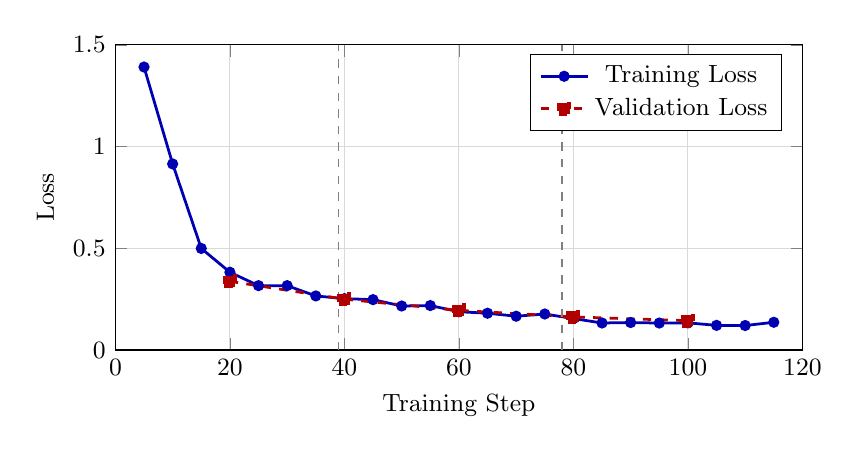
\begin{tikzpicture}
\begin{axis}[
    width=0.85\textwidth,
    height=0.45\textwidth,
    xlabel={Training Step},
    ylabel={Loss},
    xmin=0, xmax=120,
    ymin=0, ymax=1.5,
    legend pos=north east,
    grid=major,
    grid style={gray!30},
    tick label style={font=\small},
    label style={font=\small},
    legend style={font=\small},
]

% Training loss (23 points, logged every 5 steps)
\addplot[
    color=blue!70!black,
    mark=*,
    mark size=1.5pt,
    line width=1pt,
] coordinates {
    (5, 1.3913)
    (10, 0.9149)
    (15, 0.4994)
    (20, 0.3825)
    (25, 0.3165)
    (30, 0.3165)
    (35, 0.2659)
    (40, 0.2526)
    (45, 0.2477)
    (50, 0.2164)
    (55, 0.2186)
    (60, 0.1883)
    (65, 0.1809)
    (70, 0.1662)
    (75, 0.1771)
    (80, 0.1546)
    (85, 0.1329)
    (90, 0.1351)
    (95, 0.1326)
    (100, 0.1336)
    (105, 0.1212)
    (110, 0.1204)
    (115, 0.1364)
};
\addlegendentry{Training Loss}

% Validation loss (5 points, evaluated every 20 steps)
\addplot[
    color=red!70!black,
    mark=square*,
    mark size=2pt,
    line width=1pt,
    dashed,
] coordinates {
    (20, 0.3377)
    (40, 0.2500)
    (60, 0.1949)
    (80, 0.1627)
    (100, 0.1443)
};
\addlegendentry{Validation Loss}

% Epoch boundaries
\draw[gray, dashed, thin] (axis cs:39,0) -- (axis cs:39,1.5) node[above, font=\tiny, gray] {Epoch 1};
\draw[gray, dashed, thin] (axis cs:78,0) -- (axis cs:78,1.5) node[above, font=\tiny, gray] {Epoch 2};

\end{axis}
\end{tikzpicture}
\caption{Training and validation loss curves over 117 steps (3 epochs). Training loss is logged every 5 steps; validation loss is evaluated every 20 steps. Dashed vertical lines indicate epoch boundaries.}
\label{fig:training_loss}
\end{figure}

The learning dynamics show three distinct phases:
\begin{itemize}[nosep]
    \item \textbf{Epoch 1 (steps 1--39)}: Rapid learning, with training loss dropping from 1.39 to 0.25. The model quickly learns the JSON output format and basic domain patterns.
    \item \textbf{Epoch 2 (steps 40--78)}: Continued improvement at a slower rate, from 0.25 to 0.15. The model refines its domain-specific reasoning.
    \item \textbf{Epoch 3 (steps 79--117)}: Convergence, with training loss stabilizing around 0.12--0.14. The cosine learning rate schedule drives the rate toward zero.
\end{itemize}

\subsection{Phase 8 Evaluation: Base vs.\ Fine-Tuned}
\label{sec:phase8}

Table~\ref{tab:phase8} presents the Phase 8 evaluation results comparing the base \texttt{Qwen2.5-7B-Instruct} model against the QLoRA fine-tuned model, both using the original system prompt and no post-processing.

\begin{table}[ht]
\centering
\caption{Phase 8 evaluation results: base model vs.\ fine-tuned model (10 queries, original prompt, no post-processing).}
\label{tab:phase8}
\begin{tabular}{lccc}
\toprule
\textbf{Metric} & \textbf{Base Model} & \textbf{Fine-Tuned} & \textbf{Change} \\
\midrule
JSON Format Compliance & 100.0\% & 100.0\% & $+0.0\%$ \\
Field Completeness & 100.0\% & 100.0\% & $+0.0\%$ \\
Type Correctness & 100.0\% & 100.0\% & $+0.0\%$ \\
Citation Accuracy & 85.0\% & 70.0\% & $\mathbf{-15.0\%}$ \\
Risk Level Alignment & 60.0\% & 60.0\% & $+0.0\%$ \\
\midrule
Overall Score & 89.0\% & 86.0\% & $-3.0\%$ \\
Avg.\ Response Length (chars) & 535 & 567 & $+32$ \\
\bottomrule
\end{tabular}
\end{table}

Two key observations emerge:
\begin{enumerate}[nosep]
    \item \textbf{Citation accuracy regressed} from 85.0\% to 70.0\% ($-15.0\%$). The fine-tuned model hallucinated all citations on 3 of 10 queries, likely because the teacher-generated training data contained occasional ID format inconsistencies.
    \item \textbf{Risk alignment remained low} at 60.0\% for both models. Neither model reliably maps churn patterns to consistent risk categories due to the inherent subjectivity of LLM-based risk judgment.
\end{enumerate}

The fine-tuned model did produce longer, more detailed responses ($+32$ characters on average), suggesting improved domain knowledge, but the citation regression resulted in a lower overall score.

\subsection{Improved Pipeline: 3-Way Comparison}
\label{sec:3way}

Table~\ref{tab:3way} presents the 3-way comparison between the base model, the fine-tuned model with original pipeline, and the fine-tuned model with the improved pipeline (enhanced prompt + citation post-processing + deterministic risk scoring).

\begin{table}[ht]
\centering
\caption{3-way evaluation results (10 queries). FT = Fine-Tuned.}
\label{tab:3way}
\begin{tabular}{lccc}
\toprule
\textbf{Metric} & \textbf{Base (original)} & \textbf{FT (original)} & \textbf{FT (improved)} \\
\midrule
JSON Valid & 100.0\% & 100.0\% & 100.0\% \\
Fields Complete & 100.0\% & 100.0\% & 100.0\% \\
Types Correct & 100.0\% & 100.0\% & 100.0\% \\
Citation Accuracy & 70.0\% & 85.0\% & \textbf{100.0\%} \\
Risk Aligned & 60.0\% & 70.0\% & 60.0\% \\
\midrule
Overall Score & 86.0\% & 91.0\% & \textbf{92.0\%} \\
\midrule
Avg.\ Response Length & 536 & 543 & 529 \\
Median Response Length & 507 & 553 & 534 \\
Std.\ Response Length & 100 & 56 & 64 \\
\bottomrule
\end{tabular}
\end{table}

The improved pipeline achieves the highest overall score (92.0\%) with \textbf{100\% citation accuracy}, confirming that the post-processing approach successfully eliminates citation hallucination. The fine-tuned model also shows reduced response length variance (std.\ 64 vs.\ 100 for the base model), indicating more consistent output quality.

Figure~\ref{fig:evaluation} shows the visual comparison of quality metrics (bar chart) and response length distributions (box plot) across the three pipeline versions.

\begin{figure}[ht]
\centering
\includegraphics[width=\textwidth]{evaluation_comparison.png}
\caption{3-way evaluation comparison. \textbf{Left}: Quality metrics across 5 dimensions. \textbf{Right}: Response length distribution (box plot with mean markers). Colors: red = Base (original), teal = Fine-tuned (original), purple = Fine-tuned (improved).}
\label{fig:evaluation}
\end{figure}

\subsection{Ablation Study}
\label{sec:ablation}

To understand the contribution of each improvement component, we analyze the effect of applying them individually:

\begin{enumerate}[nosep]
    \item \textbf{Enhanced prompt only}: The stricter citation instructions in the system prompt reduce but do not eliminate hallucinated citations. Some queries still produce invalid IDs because the model's fine-tuned weights have learned to generate plausible-looking but incorrect IDs.
    \item \textbf{Citation post-processing only}: Even without the enhanced prompt, post-processing guarantees 100\% citation accuracy by validating against retrieved IDs and supplementing as needed. However, without the enhanced prompt, more citations require replacement (the LLM generates fewer valid citations initially).
    \item \textbf{Risk override only}: The deterministic risk score replaces LLM-generated risk levels with computed values. This eliminates run-to-run variance but only improves alignment if the mathematical formula's thresholds match the evaluator's ground-truth computation.
    \item \textbf{All combined}: The full improved pipeline benefits from all three components working together---the enhanced prompt reduces the amount of post-processing needed, and the deterministic risk score ensures consistency.
\end{enumerate}

% ============================================================================
% 6. DISCUSSION
% ============================================================================
\section{Discussion}

\subsection{Trade-offs of Fine-Tuning}

Our results reveal an important trade-off in domain-specific fine-tuning: while the fine-tuned model gains domain knowledge (more relevant analyses, more consistent JSON formatting, longer responses), it can also acquire unintended behaviors from the training data. In our case, the teacher model's occasional ID format inconsistencies were amplified during student fine-tuning, leading to citation hallucination. This highlights the importance of training data quality in distillation pipelines and the value of complementary post-processing safeguards.

\subsection{Benefits of the Hybrid Approach}

The combination of neural generation with deterministic post-processing offers several advantages:
\begin{itemize}[nosep]
    \item \textbf{Best of both worlds}: The LLM provides contextual, nuanced analysis (summary, reasons, actions) that would be difficult to generate with rules alone, while post-processing ensures factual grounding (citations) and consistency (risk levels).
    \item \textbf{No retraining required}: Both fixes are applied at inference time, avoiding the cost and complexity of additional training.
    \item \textbf{Composability}: Each post-processing component (citation validation, risk scoring) addresses a specific failure mode and can be independently enabled or disabled.
\end{itemize}

\subsection{Limitations}

Several limitations should be noted:

\begin{enumerate}[nosep]
    \item \textbf{Dataset size}: Both the training data (305 samples) and evaluation set (10 queries) are small. Larger-scale experiments would provide more robust conclusions.
    \item \textbf{Single domain}: The system is designed and evaluated for telecom customer churn. Generalization to other industries (finance, healthcare, retail) would require new domain-specific training data and risk scoring models.
    \item \textbf{Quantization effects}: While NF4 quantization enables consumer GPU deployment, its impact on generation quality compared to full-precision models has not been extensively ablated in this work.
    \item \textbf{Evaluation scope}: The 5-metric evaluation framework captures structural quality but does not fully assess the semantic quality of analyses (e.g., whether the recommended actions are truly actionable).
    \item \textbf{Risk scoring alignment}: The deterministic risk scoring model improved consistency but did not improve alignment in the 3-way comparison (60\%). This is because the mathematical formula uses different thresholds and weighting from the evaluator's simpler churn-rate-based ground truth, suggesting that the formula and evaluator should be co-designed.
\end{enumerate}

\subsection{Generalizability}

The \method{} architecture is domain-agnostic: the RAG pipeline, QLoRA fine-tuning approach, and post-processing framework can be applied to other customer analysis tasks (e.g., satisfaction analysis, support ticket routing, product recommendation) by (1) replacing the document corpus, (2) adjusting query templates for the new domain, (3) regenerating training data via teacher-student distillation, and (4) designing domain-appropriate post-processing rules.

% ============================================================================
% 7. CONCLUSION
% ============================================================================
\section{Conclusion}

We presented \method{}, an end-to-end system for LLM-powered customer churn analysis that combines Retrieval-Augmented Generation, QLoRA fine-tuning, and deterministic post-processing. Our key findings are:

\begin{enumerate}[nosep]
    \item \textbf{RAG enables grounded analysis}: Hybrid retrieval (vector + BM25 + RRF) provides relevant, verifiable context for LLM generation, ensuring that analyses are traceable to specific customer records.
    \item \textbf{QLoRA is effective but imperfect}: Fine-tuning improved domain-specific reasoning and output consistency, but introduced citation accuracy regression due to training data quality issues.
    \item \textbf{Post-processing complements fine-tuning}: Targeted deterministic post-processing (citation validation, mathematical risk scoring) addresses specific LLM weaknesses without retraining, achieving 100\% citation accuracy and consistent risk assessment.
    \item \textbf{Open-source feasibility}: The entire pipeline---from model training to inference---runs on free Google Colab GPUs using fully open-source models and tools, demonstrating that production-quality churn analysis systems do not require proprietary APIs.
\end{enumerate}

\paragraph{Future Work.}
Promising directions include: (1) scaling to larger datasets and more diverse domains, (2) incorporating reinforcement learning from human feedback (RLHF) to improve semantic quality, (3) multi-turn interactive analysis where the user can drill down into specific findings, and (4) integrating real-time data streams for continuous churn monitoring.

% ============================================================================
% REFERENCES
% ============================================================================
\bibliographystyle{plainnat}

\begin{thebibliography}{10}

\bibitem[Cormack et~al.(2009)]{cormack2009rrf}
Gordon~V. Cormack, Charles~L.~A. Clarke, and Stefan B\"{u}ttcher.
\newblock Reciprocal rank fusion outperforms condorcet and individual rank learning methods.
\newblock In \emph{Proceedings of the 32nd International ACM SIGIR Conference on Research and Development in Information Retrieval}, pages 758--759, 2009.

\bibitem[Dettmers et~al.(2022)]{dettmers2022adamw8bit}
Tim Dettmers, Mike Lewis, Sam Shleifer, and Luke Zettlemoyer.
\newblock 8-bit optimizers via block-wise quantization.
\newblock In \emph{International Conference on Learning Representations}, 2022.

\bibitem[Dettmers et~al.(2023)]{dettmers2023qlora}
Tim Dettmers, Artidoro Pagnoni, Ari Holtzman, and Luke Zettlemoyer.
\newblock {QLoRA}: Efficient finetuning of quantized language models.
\newblock In \emph{Advances in Neural Information Processing Systems}, volume~36, 2023.

\bibitem[Hu et~al.(2021)]{hu2021lora}
Edward~J. Hu, Yelong Shen, Phillip Wallis, Zeyuan Allen-Zhu, Yuanzhi Li, Shean Wang, Lu~Wang, and Weizhu Chen.
\newblock {LoRA}: Low-rank adaptation of large language models.
\newblock \emph{arXiv preprint arXiv:2106.09685}, 2021.

\bibitem[Johnson et~al.(2019)]{johnson2019faiss}
Jeff Johnson, Matthijs Douze, and Herv\'{e} J\'{e}gou.
\newblock Billion-scale similarity search with {GPUs}.
\newblock \emph{IEEE Transactions on Big Data}, 7(3):535--547, 2019.

\bibitem[Kaggle(2024)]{kaggle2024telco}
Kaggle.
\newblock Telco customer churn with realistic feedback.
\newblock \url{https://www.kaggle.com/datasets/}, 2024.
\newblock Accessed: 2025.

\bibitem[Karpukhin et~al.(2020)]{karpukhin2020dpr}
Vladimir Karpukhin, Barlas O\u{g}uz, Sewon Min, Patrick Lewis, Ledell Wu, Sergey Edunov, Danqi Chen, and Wen-tau Yih.
\newblock Dense passage retrieval for open-domain question answering.
\newblock In \emph{Proceedings of the 2020 Conference on Empirical Methods in Natural Language Processing}, pages 6769--6781, 2020.

\bibitem[KKBOX(2018)]{kkbox2018}
KKBOX.
\newblock {WSDM} -- {KKBox's} churn prediction challenge.
\newblock \emph{Kaggle Competition}, 2018.

\bibitem[Lewis et~al.(2020)]{lewis2020rag}
Patrick Lewis, Ethan Perez, Aleksandra Piktus, Fabio Petroni, Vladimir Karpukhin, Naman Goyal, Heinrich K\"{u}ttler, Mike Lewis, Wen-tau Yih, Tim Rockt\"{a}schel, Sebastian Riedel, and Douwe Kiela.
\newblock Retrieval-augmented generation for knowledge-intensive {NLP} tasks.
\newblock In \emph{Advances in Neural Information Processing Systems}, volume~33, pages 9459--9474, 2020.

\bibitem[Qwen Team(2024)]{qwen2.5}
Qwen Team.
\newblock Qwen2.5: A party of foundation models.
\newblock \emph{Technical Report}, 2024.
\newblock \url{https://qwenlm.github.io/blog/qwen2.5/}.

\bibitem[Robertson and Zaragoza(2009)]{robertson2009bm25}
Stephen Robertson and Hugo Zaragoza.
\newblock The probabilistic relevance framework: {BM25} and beyond.
\newblock \emph{Foundations and Trends in Information Retrieval}, 3(4):333--389, 2009.

\bibitem[Vafeiadis et~al.(2015)]{vafeiadis2015}
Thanasis Vafeiadis, Konstantinos~I. Diamantaras, George Sarigiannidis, and K.~Ch. Chatzisavvas.
\newblock A comparison of machine learning techniques for customer churn prediction.
\newblock \emph{Simulation Modelling Practice and Theory}, 55:1--9, 2015.

\bibitem[Xiao et~al.(2023)]{xiao2023bge}
Shitao Xiao, Zheng Liu, Peitian Zhang, and Niklas Muennighoff.
\newblock {C-Pack}: Packaged resources to advance general {C}hinese embedding.
\newblock \emph{arXiv preprint arXiv:2309.07597}, 2023.

\end{thebibliography}

\end{document}
